\documentclass{article}%
\usepackage[T1]{fontenc}%
\usepackage[utf8]{inputenc}%
\usepackage{lmodern}%
\usepackage{textcomp}%
\usepackage{lastpage}%
\usepackage[head=40pt,margin=0.5in,bottom=0.6in]{geometry}%
\usepackage{graphicx}%
%
\title{\textbf{Espacio Público ante la CIDH: Venezuela tiene una crisis económica inmensa}}%
\author{EL NACIONAL WEB}%
\date{04/10/2018}%
%
\begin{document}%
\normalsize%
\maketitle%
\textbf{URL: }%
http://www.el{-}nacional.com/noticias/mundo/espacio{-}publico{-}ante{-}cidh{-}venezuela{-}tiene{-}una{-}crisis{-}economica{-}inmensa\_254343\newline%
%
\textbf{Periodico: }%
EN, %
ID: %
254343, %
Seccion: %
Mundo\newline%
%
\textbf{Palabras Claves: }%
Mundo, Crisis económica\newline%
%
\textbf{Derecho: }%
5%
, Otros Derechos: %
18%
, Sub Derechos: %
NO\_TIENE%
\newline%
%
\textbf{EP: }%
SI\newline%
\newline%
%
\textbf{\textit{Carlos Correa alegó que el producto interno bruto ha caído por cinco años seguidos}}%
\newline%
\newline%
%
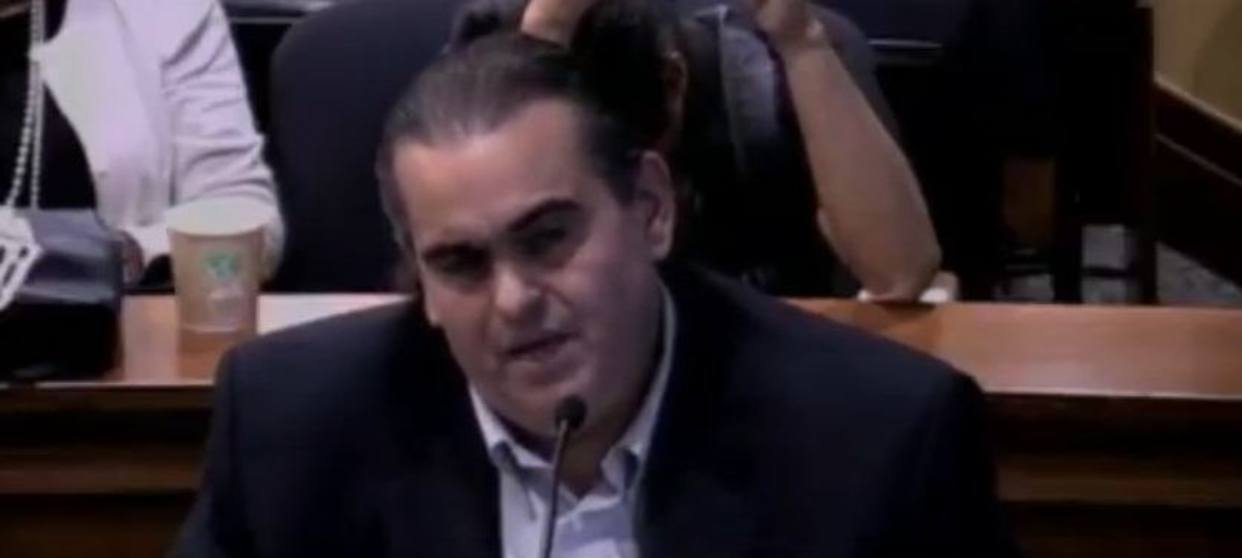
\includegraphics[width=300px]{82.jpg}%
\newline%
%
Carlos Correa, director de la organización no gubernamental Espacio Público, indicó este jueves que Venezuela está sumergida en una crisis económica severa.%
\newline%
%
"Venezuela tiene una crisis económica inmensa. Nuestro producto interno bruto~ha caído por 5 años seguidos. Tenemos la inflación más alta del mundo, pero no tenemos acceso a esta información", dijo durante~la audiencia de la Comisión Interamericana de Derechos Humanos sobre la violación de los Derechos Humanos en Venezuela.%
\newline%
%
Destacó la necesidad de mostrar la información en los ámbitos económicos y sociales~por la ausencia de cifras inflacionarias y de aprisionados, luego de que~Larry Davoe, representante de Venezuela en la audiencia de la CIDH, mostrara cifras de los casos.%
\newline%
%
Correa responsabilizó al Estado venezolano de no tener el debido control de la inflación y la ausencia de soluciones para el país.%
\newline%
%
\end{document}